% Die Software ist komplex und hat viele Abhängigkeiten. Eine Datei alleine ist nicht genug.
% Auch im Hinblick auf TPT. Es ist Stand jetzt immer noch nicht möglich das Gesamtprojekt zu analysieren.
% Eine Komponente, nämlich SCB, kann kompiliert werden. Dahingegen einzelne Dateien innerhalb der Komponente
% können widerum nicht alleine kompiliert werden. Aus diesen Gründen wurde eine C Datei 
% nachgestellt. Diese Datei soll so viele Informationen wie die reale Datei haben, jedoch
% alle Abhängigkeiten, die nicht für den Quicktest gebraucht werden.
% So wenig wie möglich, so viel wie nötig.
% Nach design pattern von ZF werden die Schnittstellen in <Komponentenname>\_Task.c definiert.
% Die Signale sind in Makros versteckt, somit benötigt das Modell eine .c Datei mit allen Makros,
% die die Signale brauchen.
% Die Software hat viele Abhängigkeiten
In diesem Kapitel wird eine C Datei für den Quicktest nachgestellt. Diese wird benutzt, um einen einfachen Schnittstellentest
in \ac{tpt} durchführen zu können. Weiterer Code aus der Datei, der nicht für den Quicktest benötigt wird, wird weggelassen.

In der Datafield stecken Informationen über die Signale und deren Schnittstellen. Um diese Schnittstelleninformationen
im Code zugreifbar zu machen, werden Makros in Header Dateien generiert. Diese Header Dateien werden durch einen include-Guard der C Datei bekannt gegeben (siehe Abbildung 4.1). Damit hat die C Datei Zugriff
auf die Schnittstellen. Die Makros werden im Code verwendet, um die Signale zu verbinden, sodass eine Schnittstelle entsteht.


% Die C Datei, in der die Schnittstelle definiert ist, hat Abhängigkeiten zu anderen Dateien, die jedoch größtenteils nicht für den Quicktest benötigt werden.
% Des Weiteren ist das Aufsetzen des Gesamtprojekts in TPT noch nicht abgeschlossen. Um ein Konzept für den Quicktest in TPT erstellen zu können, ohne dass es an Mühen für die Projekteinrichtung bedarf,
% %die Einrichtung des Softwareprojekts stört,
% wird eine C Datei nachgestellt.
% Nach design pattern von ZF werden die Schnittstellen in <Komponentenname>\_Task.c definiert. Die Wertzuweisung der Signale im Sinne der Schnittstelle sind in Makros definiert. Somit benötigt die Nachstellung eine C Datei mit 3 Makros, die in Header Dateien
% definiert sind und von der C Datei eingebunden werden, so wie hier zu sehen ist:\\
%\newpage
\begin{figure}[h]
\centering
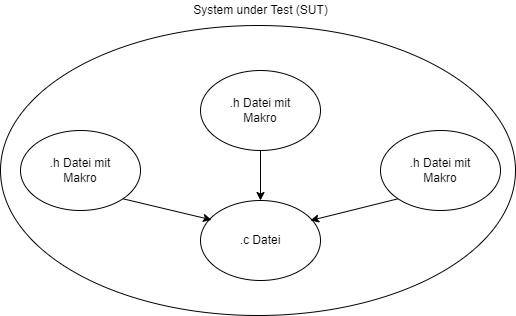
\includegraphics[scale=.6,]{Bilder/Quicktest/Makros.drawio.png}
\caption{Sourcenmodell für den Quicktest}
\end{figure}

% Es wird eine Schnittstelle in der C Datei nachgestellt (siehe Abbildung 4.1). Eine Schnittstelle besteht aus drei Makros.
% %Im Kommentar ist zu sehen, dass es eine einfache Wertzuweisung ist, wenn die Makros aufgelöst sind. 
% Es werden drei Header Dateien mit dem include-Guard eingebunden, in denen Makros stehen.   

In Listing 4.1 ist die C Datei zu sehen. Im Kommentar (Zeilen beginnend mit //) ist zu sehen, 
dass es eine einfache Wertzuweisung ist, wenn die Makros aufgelöst sind.\par
\lstinputlisting[style=customc, caption=C Datei Quicktest]{Code/TestfallmitDatafield.c}
In Listing 4.2 ist eine Header Datei zu sehen. Dieses Makro hat das Prinzip eines Setters. Ein Setter wird in der
objektorientierten Programmierung eingesetzt. Es ist eine Methode, die ein Attribut auf einen Wert setzt. Dieser Wert
wird der Methode als Parameter übergeben. Hier ist es ein Makro und es wird anstatt eines Attributs ein Signal auf einen
Wert gesetzt \parencite[S. 414 f.]{java}.

\lstinputlisting[style=customc, caption=Setter Makro]{Code/STBPrivatedfi.h}
In Listing 4.3 ist die nächste Header Datei zu sehen. Dieses Makro setzt ein weiteres Makro ein.
\lstinputlisting[style=customc, caption=Makro verweist auf ein weiteres Makro]{Code/ZIL_STB_dfi.h}
In Listing 4.4 ist die dritte Header Datei zu sehen. Dieses Makro hat das Prinzip eines Getters und kommt ähnlich
wie der vorher beschriebene Setter aus der objektorientierten Programmierung. Das Getter Makro gibt 
in diesem Fall ein Signal wieder.
\lstinputlisting[style=customc, caption=Getter Makro]{Code/SDC_Public_dfi.h}



Löst man nun alle drei Makros auf, wird wie zuvor schon erwähnt, erkenntlich, dass es eine Wertzuweisung ist. Das Setter Makro bekommt
als Parameter das Getter Makro. Der Wert
des Signals einer anderen Komponente wird in ein Signal dieser Komponente eingesetzt. Dies entspricht einer Schnittstelle.
% Es wird eine Schnittstelle in der C Datei nachgestellt(siehe Abbildung XY). Eine Schnittstelle besteht aus drei Makros.
% Im Kommentar ist zu sehen, dass es einfache Wertzuweisung ist, wenn die Makros aufgelöst sind.
% Es werden drei Header Dateien mit dem include-Guard eingebunden, in denen die Makros stehen.

% %\lstinputlisting{Code/TestfallmitDatafield.c}

% %\lstinputlisting[style=customc, caption=Schnittstelle mit Makros]{Code/TestfallmitDatafield.c}

% In Abbildung XY ist eine Header Datei zu sehen. Dieses Makro hat das Prinzip eines Setters. Eine Setter wird in der 
% objektorientierten Programmierung eingesetzt. Es ist dabei eine Methode, die ein Attribut auf einen Wert setzt. Dieser
% Wert wird der Methode als Parameter übergeben. Der Unterschied zu dem Makro ist: Der Hintergrund ist keine Klasse, sondern
% eine Header Datei. Es ist keine Methode, sondern ein Makro. Es ist kein Attribut, sondern ein Signal\parencite[S.414 f.]{java}.
% Hier ist mehr Text, passt.
% %\lstinputlisting[style=customc, caption=Schnittstelle mit Makros]{Code/STBPrivatedfi.h}
% %\lstinputlisting[style=customc, caption=SetterMakro]{Code/STBPrivatedfi.h}

% % In Abbildung XY ist die nächste Header Datei zu sehen, in dem ein Makro definiert ist.
% % Dieses Makro verweist auf ein weiteres Makro.
% % \lstinputlisting[style=customc, caption=Makro verweist auf weiteres Makro]{Code/ZIL_STB_dfi.h}

% % In Abbildung XY ist die letzte Header Datei zu sehen. Darin ist das Makro definiert, worauf das vorherige Makro verwiesen hat.
% % Dieses Makro hat das Prinzip eines Getters und kommt ähnlich wie der vorher beschriebene Setter aus der objektorientierten
% % Programmierung. Das Getter Makro gibt den Wert eines Signals wieder.
% % Löst man die Makros des Getter und des Setter auf, bekommt man eine Wertzuweisung, wie es im Kommentar in Abbildung XY zu sehen ist.
 % % % eines Signals von einer zweiten Komponente
 % % % auf das andere Signal. Das Getter Makro holt ein Signal von einer Komponente. Das Setter Makro setzt ein Signal der Komponente auf einen Wert.
% % In das Setter Makro wird als Parameter das Getter Makro eingesetzt.
% % Das Getter Makro holt den Wert eines Signals von einer anderen Komponente und dieser Wert wird durch das Setter Makro 
% % auf ein Signal in dieser Komponente gesetzt.
% % \lstinputlisting[style=customc, caption=Getter Makro]{Code/SDC_Public_dfi.h}




% % In dieser Header Datei ist das Makro SDC Public, es zeigt auf ein Signal.(Code zeigen) Getter mit java als Quelle

% % In dieser Header Datei, Makro: in dem Makro ist ist ein weiteres Makro (Header Makro in Makro zeigen)

% % in dieser Header Datei: Makro zeigt auf STB Label. Setter mit java als Quelle

% % Des Weiteren sind die Signale in einer C Datei definiert. Um diese Datei TPT bekannt zu machen, muss im TPT Wrapper diese Datei eingebunden werden.
% % Es gibt schon eine Datei namens vs\_includes intern, die alle structs der Signale einbindet. Diese wird im TPT Wrapper eingebunden.


% % Danach Code zeigen und Getter, Setter erklären.